\chapter{Namespace XML}

Les documents XML bien formés répondront à l'arborescence présentée ci-dessous.

Les hypothèse suivantes sont également formulées :
\begin{itemize}
    \item Les documents XML à parser ne contiendront pas de DTD interne
    \item Les Process Instruction (PI) ne contiendront que des attributs
    \item Aucune référence ne sera présente dans les documents XML\\
\end{itemize}


\section{Diagramme de classes}
    Les classes ici décrites seront rattachées au \lstinline$namespace Xml$ défini en C++.

    \begin{landscape}
    \begin{figure}[h!]
        \centering
        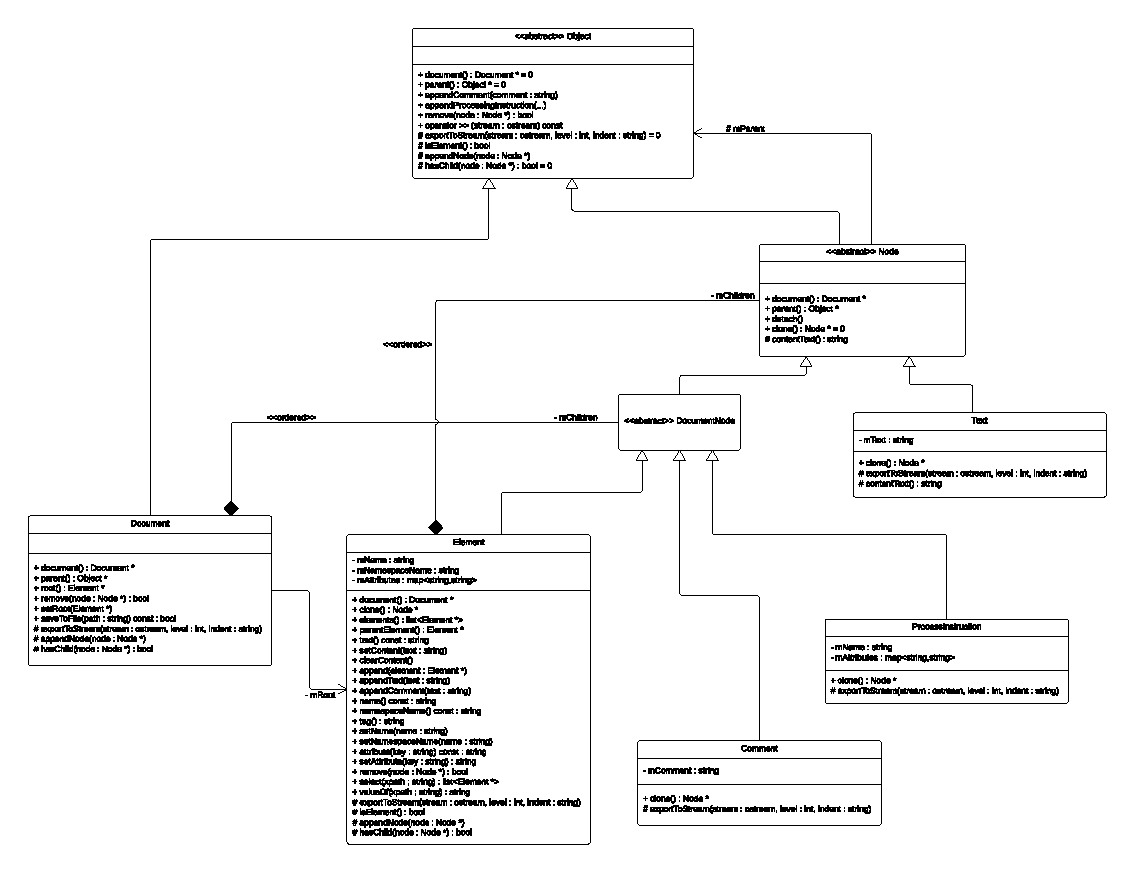
\includegraphics[width=0.9\linewidth]{images/xml-uml.pdf}
        \caption{Diagramme de classes de l'arborescence XML}
        \label{classDiagram}
    \end{figure}
    \end{landscape}


\section{Classes}
    \subsection{Log}
        La class \lstinline$Log$ a pour unique mission de stocker l'ensemble de l'output du parseur \textit{XML} telle que~:

        \begin{itemize}
            \item Erreurs lexicales~;
            \item Erreurs syntaxique~;
            \item Erreurs semantiques.
        \end{itemize}

    \subsection{Object}
        Pour optimiser et eviter au maximum la redondance de donner dans notre arbre d'h\'eritage de l'implementation \textit{XML}, nous nous somme inspirer de la tres c\'elebre librarie \textit{Qt} avec sont \lstinline$QObject$. Ainsi nous avons notre \lstinline$Xml::Object$ offrant les avantages que vous trouverez dans les sous sections suivantes.

    \subsection{Node}
        Ainsi, nous partons du principe qu'un document XML n'est en faite qu'un arbre aillant des noeux (\lstinline$Node$) \'etant des objects XML, mais de natures differents (commentaires, text, element ...). Certains de ces noeux serons des feuilles de l'arbre pour le noeux de commentaire par exemple.

        C'est la d\'ej\`a un avantage du \lstinline$Xml::Object$ car chaque \lstinline$Node$ connais sont \lstinline$Object$ parent \'a l'aide de \lstinline$mParent$ pouvant etre un \lstinline$Element$ ou un \lstinline$Document$. Ainsi, on peut \'a partir d'un noeud, retrouver le \lstinline$Document$ dans lequel il se trouve simplement en remontant l'arbre.

    \subsection{DocumentNode}
        Le \lstinline$DocumentNode$ est une sp\'ecialisation de \lstinline$Node$, mais aillant seulement une particularit\'e' s\'emantique~: seul ses classes fillent peuvent avoir pour parent, un \lstinline$Element$ par hertiage de \lstinline$Node$, mais aussi un \lstinline$Document$ au contraire de la classe \lstinline$Text$ ne pouvant avoir pour parent qu'un \lstinline$Element$.

    \subsection{Document}
        Un \lstinline$Document$ est un \lstinline$Node$ aillant une composition de \lstinline$DocumentNode$. Parmis ces \lstinline$DocumentNode$, un seul et unique \lstinline$Element$ racine compose cette liste. Mais afin de pouvoir retrouver cette racine du document en complexit\'ee $O(1)$, \lstinline$DocumentNode$ dispose aussi d'un attributs \lstinline$mRoot$ dedi\'e \`a cette tache.

        Cette m\^eme liste de \lstinline$DocumentNode$ est ordonn\'ee pour pouvoir garentir l'ordre des noeux au chargement et \`a l'export du document \textit{XML}. L'\lstinline$Element$ racine compose cette liste pour eviter de gerer deux listes de noeux (ceux avant et ceux apr\`es).

    \subsection{Comment}
        \lstinline$Comment$ est un \lstinline$DocumentNode$ car il peut \^etre n'importe ou dans le document \textit{XML}~: dans un \lstinline$Element$ ou bien en dehors de l'element racine du document.

    \subsection{ProcessingInstruction}
        Une \lstinline$ProcessingInstruction$ est aussi un \lstinline$DocumentNode$ d'apr\'es les specifications officiel de \textit{XML}. Mais en accord avec l'hypothèse énoncée précédemment, une \lstinline$ProcessingInstruction$ ne contient qu'un nom et une map d'attributs.

    \subsection{Text}
        Un noeud de texte est naturellement décrit par une chaîne de caractères \lstinline$mText$. Celui-ci ne dérive pas de la classe \lstinline$DocumentNode$ puisque, si son contenu s'apparente à celui d'un noeud Comment, il ne peut en revanche être contenu par une instance de \lstinline$Element$. D'ou la nécessit\'ee d'ajouter le niveau de spécialisation \lstinline$DocumentNode$ afin d'éviter une relation ne respectant pas les sp\'ecifications standart \textit{XML}.

    \subsection{Element}
        Un \lstinline$Element$ \textit{XML} est un \lstinline$DocumentNode$ car il poss\`ede une liste d'\lstinline$Element$ enfant \lstinline$mChildren$, mais aussi peut l'\lstinline$Element$ racine d'un \lstinline$Document$.

        Celui ci est defini avec un nom de balise (\lstinline$mName$) mais aussi d'un espace de nom (\lstinline$mNamespaceName$). La concatenation de ces deux derniers forme le tag de l'\lstinline$Element$. Le nom du membre \lstinline$mNamespaceName$ au lieu de \lstinline$mNamespace$ a \'et\'e effectuer pour eviter la colision avec le mot clef du language C++ \lstinline$namespace$ avec son getter th\'eorique \lstinline$Xml::Element::namespace()$ remplacer par \lstinline$Xml::Element::namespaceName()$.

        Un \lstinline$Element$ possede un ensemble non-ordonné d'attributs etant simplement une map aillant une assossiation $clef \leftarrow valeur$, par soucis de determinisme, nous les exportons par ordre alphabetique des clefs.

        Enfin un \lstinline$Element$ possede une liste ordonn\'ee de noeux (\lstinline$Node$). Mais cette liste est innaccessible \`a l'utilisateur. En effet, nous ne voulons pas que l'utilisateur du namespace ai besoin de tester les differents types de de noeux. Mais \lstinline$Xml::Element::elements()$ permettent de recuperer
        l'ensemble des \lstinline$Element$ fils. Mais il ne pourra pas recuperer les \lstinline$Comment$ car ne sont pas senser \^etre parser. De m\^eme l'utilisateur ne pourra acceder aux \lstinline$ProcessingInstruction$ car sont seulement dedier au parser \textit{XML}.

        Bien sur l'utilisateur peux acceder au contenu text d'un \lstinline$Element$ \`a l'aide de \lstinline$Xml::Element::text()$ qui concatenera (avec saut de lignes entre) l'ensemble des noeux enfant de type \lstinline$Text$. Seul le parser Xsl aura le droit d'acceder \`a \lstinline$Xml::Element::mChildren$ \`a l'aide d'une amiti\'e.


\section{Encapsulation du namespace Xml}
    Au final l'utilisateur aura simplement acc\`es au classes suivante~:

    \begin{itemize}
        \item \lstinline$Log$~;
        \item \lstinline$Object$~;
        \item \lstinline$Document$~;
        \item \lstinline$Element$.
    \end{itemize}

    Les autres classes sont impl\'ement\'ees avec des constructeurs \lstinline$private$ (avec des amiti\'ees n\'ecessaires entre elles bien entendu). Ainsi l'utilisateur peut reutiliser notre impl\'ementation tout aussi facilement que la librarie \lstinline$DOM$ ayant pour avantage de ne pas avoir \`a gerer la pr\'esence de commentaires ou de processing instructions dans son code car ne travaillant dans l'arbre \textit{XML} qu'avec \lstinline$Document$ et \lstinline$Element$.
    \\
    \begin{lstlisting}[frame=single]
Xml::Document doc;

doc.setRoot(new Xml::Element("root"));
doc.root()->append(new Xml::Element("hi"));
doc.root()->appendComment("Hello world!");
doc.root()->append(new Xml::Element("bar", "foo"));

assert(doc.elements("hi").size() == 1);

doc.elements()[1]->setAttribute("attr", "myValue");

delete doc.elements("hi")[0];

std::cout << doc << std::endl;
/** stdout:
 * <root>
 *   <!--Hello world!-->
 *   <foo:bar attr="myValue"/>
 * </root>
 */
    \end{lstlisting}


\section{Algorithmes}

    \subsection{Xml::Element::select}

    \textbf{\lstinline$std::list<Xml::Element const *> Xml::Element::select(std::string const \& xPathQuery) const$}

    Dans la suite de cette section, nous nous référerons à l'élément sur lequel nous appelons \lstinline$Xml::Element::select$ par "E".

    \subsubsection{Description}
    Cette méthode permet de récupérer la liste des éléments matchant une requête XPath.

    Les requêtes XPath supportées sont les suivantes :
    \begin{itemize}
        \item "" : Retourne une liste vide.
        \item "/" : Retourne une liste contenant la racine du document si E fait partie d'un document, une liste vide sinon.
        \item "." : Retourne une liste contenant E.
        \item ".." : Retourne une liste contenant le parent de E si le parent est un élément, une liste vide sinon.
        \item "bookstore" : Retourne liste des éléments enfants de E qui ont pour tag \textit{bookstore}.
        \item "bookstore/book" : Retourne la liste des éléments qui sont des \textit{book} enfants de \textit{bookstore} enfants de E.
        \item "/bookstore/book" : Retourne la liste des éléments qui sont des \textit{book} enfants de \textit{bookstore} qui sont enfants de la racine du document si E appartient à un document, une liste vide sinon.
    \end{itemize}

    \subsubsection{Algorithme}

    Pour la suite, nous nous référerons à la requête XPath par "XP".

    Le fonctionnement de l'algorithme \lstinline$Xml::Element::select$ est le suivant :
    On regarde si XP est égale à "", "/", "." ou ".." ce qui correspond aux 4 premiers cas triviaux cités précedemment.
    Si XP se trouve parmi ces 4 cas, le traitement est immédiat et retourne ce qui a été définis au-dessus.

    Sinon, on regarde si XP possède un "/" :
    \begin{itemize}
        \item Si XP ne possède pas de "/", XP est un tag simple et on cherche, parmi les éléments de E, les éléments qui ont pour tag XP et on les renvoie dans une liste.
        \item Si XP possède moins un "/" mais ne commence pas par un "/", il s'agit d'un chemin relatif par rapport à E. Dans ce cas, on extrait la chaîne partant du début de XP jusqu'au premier "/" et on récupère tous les enfants de E qui possède ce tag. Ensuite, on appelle récursivement \lstinline$Xml::Element::select$ sur chacun des éléments avec pour requête XPath la sous-chaîne de XP commençant juste après le premier "/" jusqu'à la fin de XP. On concatène ensuite toutes les listes récupérées via les appels à \lstinline$Xml::Element::select$, puis on renvoie la nouvelle liste générée.
        \item Si XP possède au moins un "/" et commence par "/", on appelle \lstinline$Xml::Element::select$ sur la racine du document contenant E avec pour requête XP privée de son premier "/". On se retrouve alors dans le cas précédent avec E étant la racine.
    \end{itemize}

    \subsection{Xml::Element::valueOf}

    \textbf{\lstinline$std::string Xml::Element::valueOf(std::string const \& xPathQuery) const$}

    \subsection{Xml::Element::matches}

    \textbf{\lstinline$bool Xml::Element::matches(std::string const \& xPathQuery) const$}
